\section{Composition of Functions} \label{S:compositionoffunctions}
\setcounter{previewactivity}{0}
%
\begin{previewactivity}[\textbf{Constructing a New Function}] \label{PA:compositionintro} \hfill \\
Let  $A = \left\{ {a, b, c, d} \right\}$, $B = \left\{ {p, q, r} \right\}$, and  
$C = \left\{ {s, t, u, v} \right\}$.  The arrow diagram in Figure~\ref{fig:preview64} shows two functions:  
$f\x A \to B$  and  $g\x B \to C$.
\begin{figure}[h]
\begin{center}
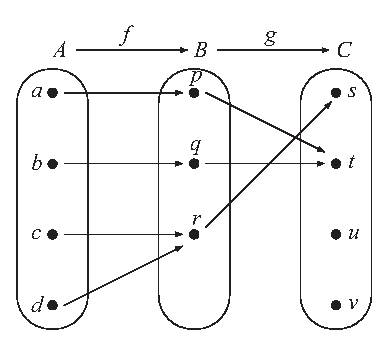
\includegraphics{figps-prev641.eps} 
\caption{Arrow Diagram Showing Two Functions} \label{fig:preview64}
\end{center}
\end{figure}
Notice that if $x \in A$, then $f(x) \in B$.  Since $f(x) \in B$, we can apply the function $g$ to $f(x)$, and we obtain 
$g(f(x))$, which is an element of $C$.

%Notice that $a \in A$ and $ f(a) = p$.  Since $p \in B$, we can use the function $g$ and obtain 
%$g(p) = t$.  This can be summarized as follows:
%\[
%g ( f(a) ) = g(p) = t.
%\]
Using this process, determine $g(f(a))$, $g ( f(b) )$, $g ( f(c) )$, and 
$g ( f(d) )$.  Then explain how we can use this information to define a function from $A$ to $C$.

%Complete the following table.  For example,  if  $x = a$, then  $f( a ) = p$, and  $g( {f( a )} ) = g( p ) = t$.
%\begin{center}
%\begin{tabular}{ c  | c | c}
% $x$  &  $f( x )$  &  $g( {f( x )} )$ \\ \hline
% $a$  &                       &                                        \\ \hline
% $b$  &                       &                                        \\ \hline
% $c$  &                       &                                        \\ \hline
% $d$  &                       &                                        \\ \hline
%\end{tabular}
%\end{center}
%Explain how this table defines a function from  $A$  to  $C$.
\end{previewactivity}
%\hbreak

\endinput

\pagebreak
\begin{previewactivity}[\textbf{Verbal Descriptions of Functions}] \label{PA:verbaldescriptions} \hfill \\
The outputs of most real functions we have studied in previous mathematics courses have been determined by mathematical expressions.  In many cases, it is possible to use these expressions to give step-by-step verbal descriptions of how to compute the outputs.  For example, if
\[
f\x \mathbb{R} \to \mathbb{R}\text{  is defined by  }f( x ) = ( {3x + 2} )^3, 
\]
we could describe how to compute the outputs as follows:

\begin{center}
\begin{tabular}{| c | l | c|}
\hline
Step  &  \textbf{Verbal Description}  &  \textbf{Symbolic Result}  \\ \hline
1  &  Choose an input.	  &  $x$           \\  \hline
2  &  Multiply by 3.	  &  $3x$          \\  \hline
3  &  Add 2.	        &  $3x + 2$      \\  \hline
4  &  Cube the result.    &  $( {3x + 2} )^3 $  \\  \hline
\end{tabular}
\end{center}
Complete step-by-step verbal descriptions for each of the following functions.
\begin{enumerate}
\item $f\x \mathbb{R} \to \mathbb{R}$ by	$f( x ) = \sqrt {3x^2  + 2} $, for each $x \in \R$.

\item $g\x \mathbb{R} \to \mathbb{R}$ by $g( x ) = \sin \! \left( {3x^2  + 2} \right)$, for each $x \in \R$.

\item $h\x \mathbb{R} \to \mathbb{R}$ by	$h( x ) = e^{3x^2  + 2} $, for each $x \in \R$.
%\item $F\x  \R \to \R$ by $F(x) = ( x^2 +3 )^3$.
%
\item $G\x  \R \to \R$ by $G(x) = \ln ( x^4 + 3 )$, for each $x \in \R$.
\item $k \x \R \to \R$ by $k(x) = \sqrt[3]{\dfrac{\sin (4x + 3)}{x^2 + 1}}$, for each $x \in \R$.
\end{enumerate}
\end{previewactivity}
\hbreak

\endinput

%\begin{previewactivity}[Constructing a New Function] \label{PA:compositionintro} \hfill \\
Let  $A = \left\{ {a, b, c, d} \right\}$, $B = \left\{ {p, q, r} \right\}$, and  
$C = \left\{ {s, t, u, v} \right\}$.  The arrow diagram in Figure~\ref{fig:preview64} shows two functions:  
$f\x A \to B$  and  $g\x B \to C$.

\begin{figure}[h]
\begin{center}
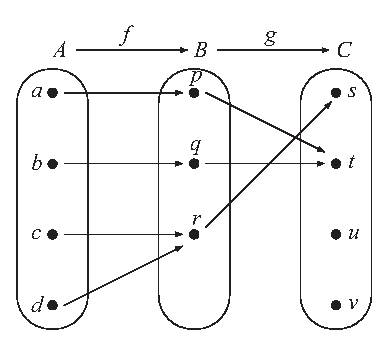
\includegraphics{figps-prev641.eps} 
\caption{Arrow Diagram Showing Two Functions} \label{fig:preview64}
\end{center}
\end{figure}
Notice that $a \in A$ and $ f(a) = p$.  Since $p \in B$, we can use the function $g$ and obtain 
$g(p) = t$.  This can be summarized as follows:
\[
g ( f(a) ) = g(p) = t.
\]
Using this process, determine $g ( f(b) )$, $g ( f(c) )$, and 
$g ( f(d) )$.  Then explain how we can now define a function from $A$ to $C$.

%Complete the following table.  For example,  if  $x = a$, then  $f( a ) = p$, and  $g( {f( a )} ) = g( p ) = t$.
%\begin{center}
%\begin{tabular}{ c  | c | c}
% $x$  &  $f( x )$  &  $g( {f( x )} )$ \\ \hline
% $a$  &                       &                                        \\ \hline
% $b$  &                       &                                        \\ \hline
% $c$  &                       &                                        \\ \hline
% $d$  &                       &                                        \\ \hline
%\end{tabular}
%\end{center}
%Explain how this table defines a function from  $A$  to  $C$.
\end{previewactivity}
\hbreak
%
\begin{previewactivity}[A New Function from Graphs] \label{PA:compositiongraphs} \hfill \\
Figure~\ref{fig:functioncomposition} shows the graphs of two real functions:  
$f\x \mathbb{R} \to \mathbb{R}$  and  $g\x \mathbb{R} \to \mathbb{R}$.  It also shows the graph of the line  $y = x$.
%\begin{figure}[h]
%\begin{center}
%\includegraphics[10.5cm,9.5cm]{figcomposition.bmp}
%\caption{Graph of $y = g( x )$ and  $y = f( x )$.} \label
%{fig:functioncomposition}
%\end{center}
%\end{figure}
\begin{figure}[h]
\begin{center}
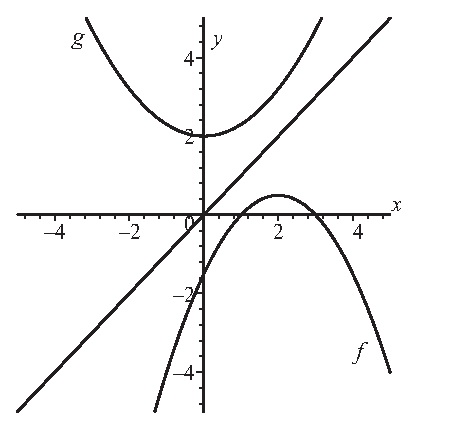
\includegraphics{figps-prev642.eps}
\caption{Graph of $y = g( x )$ and  $y = f( x )$} 
\label{fig:functioncomposition}
\end{center}
\end{figure}

%
\begin{enumerate}
\item We will first use  $x = 2$. \label{PA:compositiongraphs1}
\begin{enumerate}
  \item Draw the vertical line  $x = 2$  so that it intersects the graph of  $f$.  Label this point  $P$.  This point of intersection is  $( {2, f( 2 )} )$.  Although we could use the graph of  $f$  to approximate  $f( 2 )$, we will not do so here.
\label{PA:compositiongraphsa}

  \item Now draw a horizontal line through the point  $P$  until it intersects the  line  
$y = x$.  Call this point of intersection  $Q$.  What are the coordinates of the point  $Q$?  Each coordinate should be expressed in terms of the function  $f$\!.

  \item Next, draw a vertical line through the point  $Q$  until it intersects the graph of  
$g$.  Call this point of intersection  $R$.  What are the coordinates of the point  $R$  in terms of the functions  $f$  and  $g$?

  \item Finally, draw a horizontal line through the point  $R$  until it intersects the vertical line  $x = 2$ from Part~(\ref{PA:compositiongraphsa}).  Call this point of intersection  $S$.  What are the coordinates of the point  $S$  in terms of the functions  $f$  and  $g$.  Approximate the $y$-coordinate of the point  $S$?
\end{enumerate}

\item Repeat Part~(\ref{PA:compositiongraphs1}) starting with  $x = 3$.

\item Repeat Part~(\ref{PA:compositiongraphs1}) starting with  $x = 0$.

\item Explain how this process can be used to define a new function from  $\mathbb{R}$
to   $\mathbb{R}$.
\end{enumerate}

\end{previewactivity}
\hbreak
%
%\newpage
\begin{previewactivity}[Verbal Descriptions of Functions] \label{PA:verbaldescriptions} \hfill \\
The outputs of most real functions we have studied in previous mathematics courses have been determined by mathematical expressions.  In many cases, it is possible to use these expressions to give step-by-step verbal descriptions of how to compute the outputs.  For example, if
\[
f\x \mathbb{R} \to \mathbb{R}\text{  is defined by  }f( x ) = ( {3x + 2} )^3, 
\]
we could describe how to compute the outputs as follows:

\begin{center}
\begin{tabular}{| c | l | c|}
\hline
Step  &  \textbf{Verbal Description}  &  \textbf{Symbolic Result}  \\ \hline
1  &  Choose an input.	  &  $x$           \\  \hline
2  &  Multiply by 3.	  &  $3x$          \\  \hline
3  &  Add 2.	        &  $3x + 2$      \\  \hline
4  &  Cube the result.    &  $( {3x + 2} )^3 $  \\  \hline
\end{tabular}
\end{center}
Complete step-by-step verbal descriptions for each of the following functions.
\begin{enumerate}
\item $f\x \mathbb{R} \to \mathbb{R}$ by	$f( x ) = \sqrt {3x^2  + 2} $

\item $g\x \mathbb{R} \to \mathbb{R}$ by $g( x ) = \sin \! \left( {3x^2  + 2} \right)$

\item $h\x \mathbb{R} \to \mathbb{R}$ by	$h( x ) = e^{3x^2  + 2} $

%\item $F\x  \R \to \R$ by $F(x) = ( x^2 +3 )^3$.
%
%\item $G\x  \R \to \R$ by $G(x) = ln ( x^2 + 3 )$.
\end{enumerate}
\end{previewactivity}
\hbreak

\endinput

\begin{center}
\setlength{\unitlength}{0.5cm}
\begin{picture}(18,14)
\put(2,6.5){\oval(3,11)}
\put(8,6.5){\oval(3,11)}
\put(14,6.5){\oval(3,11)}

\put(2,2){\circle*{.5}}
\put(2,5){\circle*{.5}}
\put(2,8){\circle*{.5}}
\put(2,11){\circle*{.5}}

\put(8,5){\circle*{.5}}
\put(8,8){\circle*{.5}}
\put(8,11){\circle*{.5}}

\put(14,2){\circle*{.5}}
\put(14,5){\circle*{.5}}
\put(14,8){\circle*{.5}}
\put(14,11){\circle*{.5}}

\put(1.1,11){$a$}
\put(1.1,8){$b$}
\put(1.1,5){$c$}
\put(1.1,2){$d$}

\put(8,11.5){$p$}
\put(8,8.5){$q$}
\put(8,5.5){$r$}

\put(14.5,11){$s$}
\put(14.5,8){$t$}
\put(14.5,5){$u$}
\put(14.5,2){$v$}

\put(2,12.5){$A$}
\put(8,12.5){$B$}
\put(14,12.5){$C$}


\put(3,12.8){\vector(1,0){4.7}}
\put(9,12.8){\vector(1,0){4.7}}

\put(5,13.2){$f$}
\put(11,13.2){$g$}

\put(2.5,11){\vector(1,0){5}}
\put(2.5,8){\vector(1,0){5}}
\put(2.5,5){\vector(1,0){5}}
\put(2.5,2){\vector(2,1){5}}

\put(8.5,11){\vector(2,-1){5}}
\put(8.5,8){\vector(1,0){5}}
\put(8.5,5.3){\vector(1,1){5.3}}

\end{picture}
\end{center}


\subsection*{Composition of Functions}
There are several ways to combine two existing functions to create a new function.  For example, in calculus, we learned how to form the product and quotient of two functions and then how to use the product rule to determine the derivative of a product of two functions and the quotient rule to determine the derivative of the quotient of two functions.

The chain rule in calculus was used to determine the derivative of the composition of two functions, and in this section,  we will focus only on the composition of two functions.  We will then consider some results about the compositions of injections and surjections.

The basic idea of function composition is that when possible, the output of a function  $f$  is used as the input of a function  $g$.  This can be referred to as ``$f$  followed by  $g$'' and is called the composition of  $f$  and  $g$. In previous mathematics courses, we used this idea to determine a formula for the composition of two real functions.

For example, if
\[
f( x ) = 3x^2  + 2 \quad \text{and} \quad g( x ) = \sin x, 
\]
then we can compute  $g( f( x ) )$  as follows:
\[
\begin{aligned}
  \hfill g( {f( x )} ) &= g \! \left( {3x^2  + 2} \right) \\
                       &= \sin \! \left( {3x^2  + 2} \right). \\ 
\end{aligned} 
\]
In this case,  $f( x )$, the output of the function  $f$, was used as the input for the function  $g$.  We now give the formal definition of the composition of two functions.  
\begin{defbox}{functioncomposition}{Let  $A$, $B$, and  $C$  be nonempty sets, and let  
$f\x A \to B$  and  $g\x B \to C$  be functions.  The \textbf{composition of}
\index{composition of functions}%
\index{function!composition}%
  $\boldsymbol{f}$ \textbf{and} $\boldsymbol{g}$  is the function  $g \circ f\x A \to C$  defined by
\label{sym:composition}
\[
( {g \circ f} )( x ) = g\left( {f( x )} \right)
\]
for all  $x \in A$.  We often refer to the function  $g \circ f$ as a \textbf{composite function}.
\index{function!composite}%
\index{composite function}%
}
\end{defbox}
It is helpful to think of the composite function  $g \circ f$
 as  ``$\boldsymbol{f}$  \textbf{followed by}  $\boldsymbol{g}$.''  We then refer to  $f$  as the \textbf{inner function}
\index{inner function}%
\index{composition of functions!inner function}%
 and  $g$  as the \textbf{outer function}.
\index{outer function}%
\index{composition of functions!outer function}%


%\begin{prog}[\textbf{Order of the Composition of Two Functions}] \label{pr:composeorder} \hfill \\
%Let  $h\x \mathbb{R} \to \mathbb{R}$ be defined by  $h( x ) = 3x + 2$ and  $g\x \mathbb{R} \to \mathbb{R}$ be defined by  $g( x ) = x^3 $.  Determine formulas for the composite functions  $g \circ h$  and  $h \circ g$.  What does this tell you about the operation of composition of functions?
%\end{prog}
%\hbreak

\subsection*{Composition and Arrow Diagrams} 
The concept of the composition of two functions can be illustrated with arrow diagrams when the domain and codomain of the functions are small, finite sets.  Although the term ``composition'' was not used then, this was done in \typeu Activity~\ref*{PA:compositionintro}, and another example is given here.

Let  $A = \left\{ {a, b, c, d} \right\}$, $B = \left\{ {p, q, r} \right\}$, and  
$C = \left\{ {s, t, u, v} \right\}$.  The arrow diagram in Figure~\ref{fig:arrow64-1} shows two functions:  
$f\x A \to B$  and  $g\x B \to C$.
\begin{figure}[h]
\begin{center}
\scalebox{0.95}{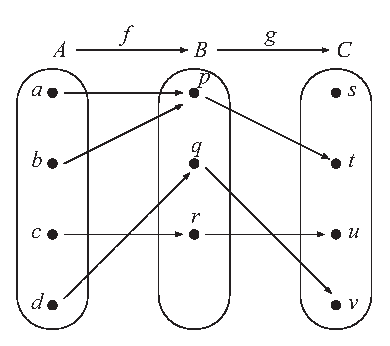
\includegraphics{figps-sec641.eps}} 
\caption{Arrow Diagram for Two Functions} \label{fig:arrow64-1}
\end{center}
\end{figure}

If we follow the arrows from the set  $A$  to the set  $C$, we will use the outputs of  $f$  as inputs of  $g$, and get the arrow diagram from  $A$  to  $C$ shown in Figure~\ref{fig:arrow64-2}.  This diagram represents the composition of  $f$  followed by  $g$.
\begin{figure}[h]
\begin{center}
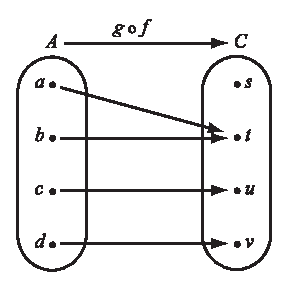
\includegraphics{figps-sec642.eps} 
\caption{Arrow Diagram for $g \circ f\x  A \to C$} \label{fig:arrow64-2}
\end{center}
\end{figure}
%
%


%\pagebreak
\begin{prog}[\textbf{The Composition of Two Functions}] \label{pr:compose} \hfill \\
Let $A = \{ a, b, c, d \}$ and $B = \{ 1, 2, 3 \}$.  Define the functions $f$ and $g$ as follows:
\begin{list}{}
\item $f \x A \to B$ defined by $f(a) = 2$, $f(b) = 3$, $f(c) = 1$, and $f(d) = 2$.
\item $g \x B \to B$ defined by $g(1) = 3$, $g(2) = 1$, and $g(3) = 2$.
\end{list}

\newpar
Create arrow diagrams for the functions $f$, $g$, $g \circ f$, and $g \circ g$.
\end{prog}
\hbreak



\endinput

\subsection*{Decomposing Functions} \index{decomposing functions}%

We use the \textbf{chain rule}
\index{chain rule}%
 in calculus to find the derivative of a composite function.  The first step in the process is to recognize a given function as a composite function.  This can be done in many ways, but the work in \typeu Activity~\ref*{PA:verbaldescriptions} can be used to decompose a function in a way that works well with the chain rule.  The use of the terms ``inner function'' and ``outer function'' can also be helpful.  The idea is that we use the last step in the process to represent the outer function, and the steps prior to that to represent the inner function.  So for the function, 
\[
f\x \mathbb{R} \to \mathbb{R}\text{  by  }f( x ) = ( {3x + 2} )^3 ,
\]
the last step in the verbal description table was to cube the result.  This means that we will use the function  $g$ (the cubing function) as the outer function and will use the prior steps as the inner function.  We will denote the inner function by  $h$.  So we let  $h\x \R \to \R$ by  
$h( x ) = 3x + 2$ and  $g\x \R \to \R$ by  $g( x ) = x^3 $.  Then
\begin{align*}
  ( {g \circ h} )( x ) &= g\left( {h( x )} \right) \\ 
                       &= g( {3x + 2} ) \\ 
                       &= ( {3x + 2} )^3  \\ 
                       &= f( x ). \\ 
\end{align*}
We see that  $g \circ h = f$\! and, hence, we have  ``decomposed''  the function  $f$.  It should be noted that there are other ways to write the function $f$ as a composition of two functions, but the way just described is the one that works well with the chain rule.  In this case, the chain rule gives
\begin{align*}
f'(x) &= ( g \circ h )'(x) \\
      &= g'(h(x))\; h'(x) \\
      &= 3(h(x))^2 \cdot 3 \\
      &= 9 (3x + 2)^2
\end{align*}
%\hbreak

\begin{prog}[\textbf{Decomposing Functions}] \label{prog:decompose} \hfill \\
Write each of the following functions as the composition of two functions.

\begin{enumerate}
%\item $f\x \mathbb{R} \to \mathbb{R}$ defined by $f( x ) = \sqrt {3x^2  + 2} $.
%
%\item $g\x \mathbb{R} \to \mathbb{R}$ defined by 
%$g( x ) = \sin ( {3x^2  + 2} )$.
%
%\item $h\x \mathbb{R} \to \mathbb{R}$ defined by $h( x ) = e^{3x^2  + 2} $.
%
%\item $k\x \mathbb{R} \to \mathbb{R}$ defined by 
%$k( x ) = \ln ( {3x^2  + 2} )$.

\item $F\x  \R \to \R$ by $F(x) = ( x^2 +3 )^3$

\item $G\x  \R \to \R$ by $G(x) = \ln ( x^2 + 3 )$

\item $f\x  \Z \to \Z$ by $f(x) = | x^2 - 3 |$

\item $g\x  \R \to \R$ by $g(x) = \cos \! \left( \dfrac{2x-3}{x^2+1} \right)$

\end{enumerate}

%\item Let  $h\x \mathbb{R} \to \mathbb{R}$ be defined by  $h( x ) = 3x + 2$ and  $g\x \mathbb{R} \to \mathbb{R}$ be defined by  $g( x ) = x^3 $.  Determine formulas for the composite functions  $g \circ h$  and  $h \circ g$.  What does this tell you about the operation of composition of functions?
%\end{enumerate}
\end{prog}
\hbreak


\endinput


\subsection*{Theorems about Composite Functions}
If $f \x A \to B$ and $g \x B \to C$, then we can form the composite function $g \circ f \x A \to C$.  In Section~\ref{S:typesoffunctions}, we learned about injections and surjections.  We now explore what type of function $g \circ f$ will be if the functions $f$ and $g$ are injections (or surjections).  

\begin{prog}[\textbf{Compositions of Injections and Surjections}] \label{prog:compositesofinjections} \hfill \\
Although other representations of functions can be used, it will be helpful to use arrow diagrams to represent the functions in this progress check.  We will use the following sets:
\[
A = \{ a, b, c \}, \quad B = \{p, q, r\}, \quad C = \{u, v, w, x \}, \quad \text{and} \quad D = \{u, v \}.
\]
\begin{enumerate}
  \item Draw an arrow diagram for a function $f \x A \to B$ that is an injection and an arrow diagram for a function $g \x B \to C$ that is an injection.  In this case, is the composite function 
$g \circ f \x A \to C$ an injection?  Explain.

    \item Draw an arrow diagram for a function $f \x A \to B$ that is a surjection and an arrow diagram for a function $g \x B \to D$ that is a surjection.  In this case, is the composite function 
$g \circ f \x A \to D$ a surjection?  Explain.

  \item Draw an arrow diagram for a function $f \x A \to B$ that is a bijection and an arrow diagram for a function $g \x B \to A$ that is a bijection.  In this case, is the composite function 
$g \circ f \x A \to A$ bijection?  Explain.
\end{enumerate}
\end{prog}
\hbreak

%
In Progress Check~\ref{prog:compositesofinjections}, we explored some properties of composite functions related to injections, surjections, and bijections.  The following theorem contains results that these explorations were intended to illustrate.  Some of the proofs will be included in the exercises.

\begin{theorem} \label{T:compositefunctions}
Let  $A$, $B$, and  $C$  be nonempty sets and assume that $f\x A \to B$ and 
$g\x B \to C$.

\begin{enumerate}
\item If  $f$  and  $g$  are both injections, then  $(g \circ f) \x A \to C$  is an injection. 
\label{T:compositefunctions1}

\item If  $f$  and  $g$  are both surjections, then  $(g \circ f) \x A \to C$  is a surjection. \label{T:compositefunctions2}

\item If  $f$  and  $g$  are both bijections, then  $(g \circ f) \x A \to C$  is a bijection. \label{T:compositefunctions3}
\end{enumerate}
\end{theorem}
%\hbreak
%
The proof of Part~(\ref{T:compositefunctions1}) is Exercise~(\ref{exer:compositefunctions1}).   Part~(\ref{T:compositefunctions3}) is a direct consequence of the first two parts.  We will discuss a process for constructing a proof  of Part~(\ref{T:compositefunctions2}).  Using the forward-backward process, we first look at the conclusion of the conditional statement in Part~(\ref{T:compositefunctions2}).  The goal is to prove that  $g \circ f$  is a surjection.  Since  $g \circ f\x A \to C$, this is equivalent to proving that

\begin{center}
For all  $c \in C$, there exists an  $a \in A$  such that  
$( {g \circ f} )( a ) = c$.
\end{center}

Since this statement in the backward process uses a universal quantifier, we will use the choose-an-element method and choose an arbitrary element $c$ in the set $C$.  The goal now is to find an  $a \in A$  such that  
$( {g \circ f} )( a ) = c$.

Now we can look at the hypotheses.  In particular, we are assuming that both  $f\x A \to B$  and  $g\x B \to C$  are surjections.  Since  we have chosen  $c \in C$,  and  $g\x B \to C$  is a surjection, we know that

\begin{center}
there exists a  $b \in B$  such that  $g( b ) = c$.
\end{center}

\noindent
Now, $b \in B$  and   $f\x A \to B$  is a surjection.  Hence

\begin{center}
there exists an  $a \in A$  such that  $f( a ) = b$.
\end{center}

\noindent
If we now compute  $( {g \circ f} )( a )$, we will see that
\[
( {g \circ f} )( a ) = g \left( f ( a ) \right) = g ( b ) = c.
\]
We can now write the proof as follows:
\eighth

%\pagebreak
\noindent
\textbf{Proof of Theorem~\ref{T:compositefunctions}, Part~(\ref{T:compositefunctions2}).}
%\begin{myproof}
Let  $A$, $B$, and  $C$  be nonempty sets and assume that  $f\x A \to B$  and  $g\x B \to C$  are both surjections.  We will prove that  $g \circ f\x A \to C$  is a surjection.
%\vskip10pt
%\noindent

Let  $c$ be an arbitrary element of  $C$.  We will prove there exists an $a \in A$ such that 
$( g \circ f ) ( a ) = c$.  Since  $g\x B \to C$  is a surjection, we conclude that

\begin{center}
there exists a  $b \in B$  such that  $g( b ) = c$.
\end{center}

\noindent
Now, $b \in B$  and   $f\x A \to B$  is a surjection.  Hence 

\begin{center}
there exists an  $a \in A$  such that  $f( a ) = b$.
\end{center}

\noindent
We now  see that
\[
\begin{aligned}
  ( {g \circ f} )( a ) &= g\left( {f( a )} \right) \\ 
                       &= g( b ) \\ 
                       &= c. \\ 
\end{aligned} 
\]
We have now shown that for every  $c \in C$, there exists an  $a \in A$  such that  $( {g \circ f} )( a ) = c$, and this proves that  $g \circ f$  is a surjection. \qed
%\end{myproof}
%\hbreak

Theorem~\ref{T:compositefunctions} shows us that if $f$ and $g$ are both special types of functions, then the composition of $f$ followed by $g$ is also that type of function.  The next question is, ``If the composition of $f$ followed by $g$ is an injection (or surjection), can we make any conclusions about $f$ or $g$?''  A partial answer to this question is provided in Theorem~\ref{T:morecompositefunctions}.  This theorem will be investigated and proved in the Explorations and Activities for this section.  See 
Exercise~(\ref{exer:morecompositefunctions1}).

\begin{theorem} \label{T:morecompositefunctions}
Let  $A$, $B$, and $C$ be nonempty sets and assume that $f\x A \to B$ and  $g\x B \to C$.

\begin{enumerate}
\item If  $g \circ f\x A \to C$  is an injection, then  $f\x A \to B$  is an injection. \label{T:morecompositefunctions1}

\item If  $g \circ f\x A \to C$ is a surjection, then  $g\x B \to C$ is a surjection. \label{T:morecompositefunctions2}
\end{enumerate}
\end{theorem}

\endinput

\begin{activity}[Exploring Composite Functions] \label{A:exploringcomposites} \hfill \\
%Although other representations of functions can be used, it might be helpful to use arrow diagrams to represent the functions in this activity.  When possible, use an example where the finite domains and codomains have different numbers of elements.
Let  $A$, $B$, and  $C$  be nonempty sets and let  $f\x A \to B$  and  $g\x B \to C$.  For this activity, it may be useful to draw your arrow diagrams in a triangular arrangement as follows:

\begin{figure}[h]
\begin{center}
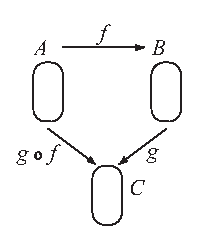
\includegraphics{figps-comparrow.eps}
%\caption{Composition of Functions} \label{fig:functioncomposition2}
\end{center}
\end{figure}

\begin{enumerate}
\item Is it possible to construct an example where  $g \circ f$  is an injection,  $f$  is an injection, but  $g$  is not an injection?  Either construct such an example or explain why it is not possible.

\item Is it possible to construct an example where  $g \circ f$  is an injection,  $g$  is an injection, but  $f$  is not an injection?  Either construct such an example or explain why it is not possible.

\item Is it possible to construct an example where  $g \circ f$  is a surjection,  $f$  is a surjection, but  $g$  is not a surjection?  Either construct such an example or explain why it is not possible.

\item Is it possible to construct an example where  $g \circ f$  is surjection,  $g$  is a surjection, but  $f$  is not a surjection?  Either construct such an example or explain why it is not possible.
\end{enumerate}
%
%\subsection*{Theorems about Composite Functions}\index{composite function!theorems about}
%In the previous two activities, we explored some properties of composite functions related to injections, surjections, and bijections.  The following two theorems contain results that these explorations were intended to illustrate.  Many of the proofs will be included in the exercises.
%
%\begin{theorem} \label{T:compositefunctions}
%Let  $A$, $B$, and  $C$  be nonempty sets and let  $f\x A \to B$ and  $g\x B \to C$.
%
%\begin{enumerate}
%\item If  $f$  and  $g$  are both injections, then  $g \circ f$  is an injection. \label{T:compositefunctions1}
%
%\item If  $f$  and  $g$  are both surjections, then  $g \circ f$  is a surjection. \label{T:compositefunctions2}
%
%\item If  $f$  and  $g$  are both bijections, then  $g \circ f$  is a bijection. \label{T:compositefunctions3}
%\end{enumerate}
%\end{theorem}
%%\hbreak
%%
%The results of Theorem~\ref{T:compositefunctions} are related to the explorations in Activity~\ref{A:compositesofinjections}.  Part~(\ref{T:compositefunctions3}) of Theorem~\ref{T:compositefunctions} is a direct consequence of the first two parts.  We will discuss constructing a proof  of Part~(\ref{T:compositefunctions2}).  Using the forward-backward process, we first look at the conclusion of the conditional statement in Part~(\ref{T:compositefunctions2}).  The goal is to prove that  $g \circ f$  is a surjection.  Since  $g \circ f\x A \to C$, this is equivalent to proving that
%
%\begin{center}
%For all  $c \in C$, there exists an  $a \in A$  such that  
%$( {g \circ f} )( a ) = c$.
%\end{center}
%
%Since this statement in the backward process uses a universal quantifier, we will start by selecting an arbitrary element $c$ in the set $C$.  The goal now is to find an  $a \in A$  such that  $( {g \circ f} )( a ) = c$.
%
%Now we can look at the hypotheses.  In particular, we are assuming that both  $f\x A \to B$  and  $g\x B \to C$  are surjections.  
%
%Since  we have chosen  $c \in C$,  and  $g\x B \to C$  is a surjection, we know that
%
%\begin{center}
%there exists a  $b \in B$  such that  $g( b ) = c$.
%\end{center}
%
%Now, $b \in B$  and   $f\x A \to B$  is a surjection.  Hence
%
%\begin{center}
%there exists an  $a \in A$  such that  $f( a ) = b$.
%\end{center}
%
%If we now compute  $( {g \circ f} )( a )$, we will see that
%\[
%( {g \circ f} )( a ) = g ( f ( a ) ) = g ( b ) = c.
%\]
%We can now write the proof as follows:
%%
%
%\pagebreak
%\noindent
%\textbf{Proof of Theorem~\ref{T:compositefunctions}, Part~(\ref{T:compositefunctions2}).}
%\begin{myproof}
%Let  $A$, $B$, and  $C$  be nonempty sets and assume that  $f\x A \to B$  and  $g\x B \to C$  are both surjections.  We will prove that  $g \circ f\x A \to C$  is a surjection.
%%\vskip10pt
%%\noindent
%
%Let  $c$ be an arbitrary element of  $C$.  We will prove there exists an $a \in A$ such that 
%$( g \circ f ) ( a ) = c$.  Since  $g\x B \to C$  is a surjection, we conclude that
%
%\begin{center}
%there exists a  $b \in B$  such that  $g( b ) = c$.
%\end{center}
%
%\noindent
%Now, $b \in B$  and   $f\x A \to B$  is a surjection.  Hence 
%
%\begin{center}
%there exists an  $a \in A$  such that  $f( a ) = b$.
%\end{center}
%
%\noindent
%We now  see that
%\[
%\begin{aligned}
%  ( {g \circ f} )( a ) &= g( {f( a )} ) \\ 
%                                             &= g( b ) \\ 
%                                             &= c. \\ 
%\end{aligned} 
%\]
%We have now shown that for every  $c \in C$, there exists an  $a \in A$  such that  $( {g \circ f} )( a ) = c$, and this proves that  $g \circ f$  is a surjection.
%\end{myproof}
%\hbreak
%
The results of Theorem~\ref{T:morecompositefunctions} are related to the explorations in Activity~\ref{A:exploringcomposites}.  The proof Theorem~\ref{T:morecompositefunctions} is 
Exercise~(\ref{exer:morecompositefunctions1}).

\begin{theorem} \label{T:morecompositefunctions}
Let  $A$, $B$, and $C$ be nonempty sets and assume that $f\x A \to B$ and  $g\x B \to C$.

\begin{enumerate}
\item If  $g \circ f\x A \to C$  is an injection, then  $f\x A \to B$  is an injection. \label{T:morecompositefunctions1}

\item If  $g \circ f\x A \to C$ is a surjection, then  $g\x B \to C$ is a surjection. \label{T:morecompositefunctions2}
\end{enumerate}
\end{theorem}
\end{activity}
\hbreak

\endinput


%
\endinput


There are several ways to combine two existing functions to create a new function.  In this section, we will focus on one way, the composition of two functions.  We will also consider some results about the compositions of injections and surjections.

\subsection*{Composition of Functions}
The basic idea of function composition is that when possible, the output of a function  $f$  is used as the input of a function  $g$.  This can be referred to as ``$f$  followed by  $g$'' and is called the composition of  $f$  and  $g$. 

The idea of the composition of two real functions is familiar from previous mathematics courses.  For example, if  $f( x ) = 3x^2  + 2$ and  
$g( x ) = \sin x$, then we can compute  $g( {f( x )} )$
 as follows:
\[
\begin{aligned}
  \hfill g( {f( x )} ) &= g \! \left( {3x^2  + 2} \right) \\
                       &= \sin \! \left( {3x^2  + 2} \right). \\ 
\end{aligned} 
\]
In this case,  $f( x )$, the output of the function  $f$, was used as the input for the function  $g$.  This idea of using the output from one function as the input for another function can be illustrated nicely with arrow diagrams.  This was done in Preview Activity~\ref{PA:compositionintro}, and another example is given here.

Let  $A = \left\{ {a, b, c, d} \right\}$, $B = \left\{ {p, q, r} \right\}$, and  
$C = \left\{ {s, t, u, v} \right\}$.  The arrow diagram in Figure~\ref{fig:arrow64-1} shows two functions:  
$f\x A \to B$  and  $g\x B \to C$.
\begin{figure}[h]
\begin{center}
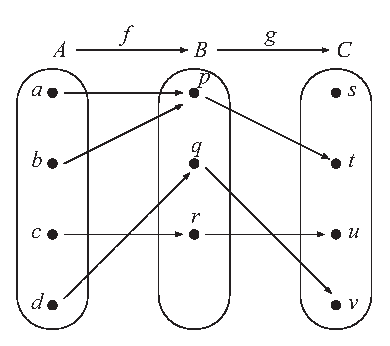
\includegraphics{figps-sec641.eps} 
\caption{Arrow Diagram for Two Functions} \label{fig:arrow64-1}
\end{center}
\end{figure}

If we follow the arrows from the set  $A$  to the set  $C$, we will use the outputs of  $f$  as inputs of  $g$, and get the arrow diagram from  $A$  to  $C$ shown in Figure~\ref{fig:arrow64-2}.  This diagram represents the composition of  $f$  and  $g$  and is denoted by  $g \circ f$\!.
\begin{figure}[h]
\begin{center}
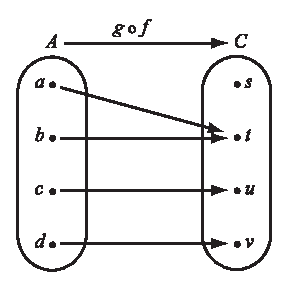
\includegraphics{figps-sec642.eps} 
\caption{Arrow Diagram for $g \circ f\x  A \to C$} \label{fig:arrow64-2}
\end{center}
\end{figure}
%
\begin{defbox}{functioncomposition}{Let  $A$, $B$, and  $C$  be nonempty sets, and let  
$f\x A \to B$  and  $g\x B \to C$  be functions.  The \textbf{composition of}
\index{composition of functions}%
\index{function!composition}%
  $\boldsymbol{f}$ \textbf{and} $\boldsymbol{g}$  is the function  $g \circ f\x A \to C$  defined by
\label{sym:composition}
\[
( {g \circ f} )( x ) = g\left( {f( x )} \right)
\]
for all  $x \in A$.  We often refer to the function  $g \circ f$ as a \textbf{composite function}.
\index{function!composite}%
\index{composite function}%
}
\end{defbox} 
%
It is helpful to think of the composite function  $g \circ f$
 as  ``$\boldsymbol{f}$  \textbf{followed by}  $\boldsymbol{g}$.''  We then refer to  $f$  as the \textbf{inner function}
\index{inner function}%
\index{composition of functions!inner function}%
 and  $g$  as the \textbf{outer function}.
\index{outerfunction}%
\index{composition of functions!outer function}%

In Preview Activity~\ref{PA:compositiongraphs}, we actually used the graphs of the real functions  $f$  and  $g$  to construct outputs for the composite function $g \circ f$.  Following is an outline of the procedure for finding $g( {f( x )} )$ for a given value of  $x$.  Figure~\ref{fig:functioncomposition2} will be used to illustrate the process.

\begin{figure}[h]
\begin{center}
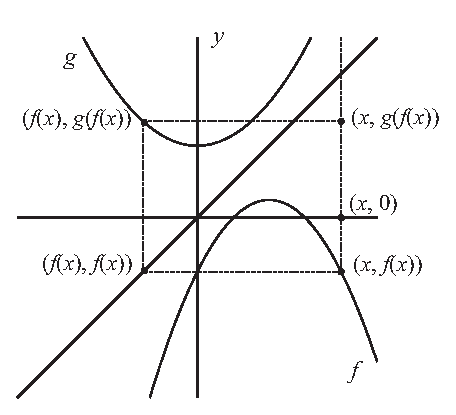
\includegraphics{figps-composition.eps}
\caption{Composition of Functions} \label{fig:functioncomposition2}
\end{center}
\end{figure}

\begin{itemize}
\item We start with an input (labeled  $x$  on the $x$-axis).  The vertical line through  $( {x, 0} )$ intersects the graph of  $f$  at the point  
$\left( {x, f( x )} \right)$.  

\item Then the horizontal line through this point intersects the line  $y = x$ at the point  
$\left( {f( x ), f( x )} \right)$.  

\item The vertical line through this point will intersect the graph of  $g$  at the point  
$\left( {f( x ), g( {f( x )} )} \right)$.  So the $y$-coordinate of this point is the output of the composite function  $g \circ f$\!.  Notice that the use of the line  $y = x$  allowed us to use the output of the function  $f$  as the input for the function  $g$.  

\item In order to obtain a point on the graph of  $y = g\left( {f( x )} \right)$, we now draw a horizontal line from the point  
$\left( {f( x ), g( {f( x )} )} \right)$ until it intersects the vertical line through the point  $( {x, 0} )$.  

\item The coordinates of this point will be  $\left( {x, g( {f( x )} )} \right)$, and hence this will be a point on the graph  of  $g \circ f$\!.
\end{itemize}
%\hrule
%
%\begin{activity}[Decomposing Functions] \label{A:decomposingfunctions} \hfill
\subsection*{Decomposing Functions} \index{decomposing functions}%


We use the \textbf{chain rule}
\index{chain rule}%
 in calculus to find the derivative of a composite function.  The first step in the process is to recognize a given function as a composite function.  This can be done in many ways, but the work in Preview Activity~\ref{PA:verbaldescriptions} can be used to decompose a function in a way that works well with the chain rule.  The use of the terms ``inner function'' and ``outer function'' can also be helpful.  The idea is that the last step in the process represents the outer function, and the steps prior to that represent the inner function.  So for the function, 
\[
f\x \mathbb{R} \to \mathbb{R}\text{  by  }f( x ) = ( {3x + 2} )^3 ,
\]
the last step in the verbal description table was to cube the result.  This means that the outer function  $g$  is the cubing function, and the prior steps are the inner function.  We will denote the inner function by  $h$.  So we let  $h\x \mathbb{R} \to \mathbb{R}$ by  
$h( x ) = 3x + 2$ and  $g\x \mathbb{R} \to \mathbb{R}$ by  $g( x ) = x^3 $.  Then
\[
\begin{aligned}
  ( {g \circ h} )( x ) &= g\left( {h( x )} \right) \\ 
                       &= g( {3x + 2} ) \\ 
                       &= ( {3x + 2} )^3  \\ 
                       &= f( x ). \\ 
\end{aligned} 
\]
We see that  $g \circ h = f$\! and, hence, we have  ``decomposed''  the function  $f$.
\hbreak

\begin{prog}[Decomposing Functions] \label{prog:decompose} \hfill
\begin{enumerate}
\item Write each of the following functions as the composition of two functions.

\begin{enumerate}
%\item $f\x \mathbb{R} \to \mathbb{R}$ defined by $f( x ) = \sqrt {3x^2  + 2} $.
%
%\item $g\x \mathbb{R} \to \mathbb{R}$ defined by 
%$g( x ) = \sin ( {3x^2  + 2} )$.
%
%\item $h\x \mathbb{R} \to \mathbb{R}$ defined by $h( x ) = e^{3x^2  + 2} $.
%
%\item $k\x \mathbb{R} \to \mathbb{R}$ defined by 
%$k( x ) = \ln ( {3x^2  + 2} )$.

\item $F\x  \R \to \R$ by $F(x) = ( x^2 +3 )^3$

\item $G\x  \R \to \R$ by $G(x) = \ln ( x^2 + 3 )$

\item $f\x  \Z \to \Z$ by $f(n) = | x^2 - 3 |$

\item $g\x  \R \to \R$ by $g(x) = \cos \! \left( \dfrac{2x-3}{x^2+1} \right)$

\end{enumerate}

\item Let  $h\x \mathbb{R} \to \mathbb{R}$ be defined by  $h( x ) = 3x + 2$ and  $g\x \mathbb{R} \to \mathbb{R}$ be defined by  $g( x ) = x^3 $.  Determine formulas for the composite functions  $g \circ h$  and  $h \circ g$.  What does this tell you about the operation of composition of functions?
\end{enumerate}
\end{prog}
%\end{activity}
\hbreak
%
\begin{prog}[Compositions of Injections and Surjections] \label{prog:compositesofinjections} \hfill \\
Although other representations of functions can be used, it might be helpful to use arrow diagrams to represent the functions in this activity.  In particular, it may be useful to use arrow diagrams similar to the one in Preview Activity~\ref{PA:compositionintro}, except that when possible, draw arrow diagrams where the three finite sets have different numbers of elements.

\begin{enumerate}
\item Construct sets $A$, $B$, and $C$ and functions $f\x A \to B$ and $g\x B \to C$, where both $f$ and $g$ are injections.  In this case, what type of function is the composite function 
$g \circ f$?

\item Construct sets $A$, $B$, and $C$ and functions $f\x A \to B$ and $g\x B \to C$, where both $f$ and $g$ are surjections.  In this case, what type of function is the composite function 
$g \circ f$?

\item Construct sets $A$, $B$, and $C$ and functions $f\x A \to B$ and $g\x B \to C$, where both $f$ and $g$ are bijections.  In this case, what type of function is the composite function $g \circ f$?
\end{enumerate}
\end{prog}
\hbreak
%
\subsection*{Theorems about Composite Functions}
In Progress Check~\ref{prog:compositesofinjections}, we explored some properties of composite functions related to injections, surjections, and bijections.  The following theorem contains results that these explorations were intended to illustrate.  Some of the proofs will be included in the exercises.

\begin{theorem} \label{T:compositefunctions}
Let  $A$, $B$, and  $C$  be nonempty sets and assume that $f\x A \to B$ and 
$g\x B \to C$.

\begin{enumerate}
\item If  $f$  and  $g$  are both injections, then  $g \circ f$  is an injection. 
\label{T:compositefunctions1}

\item If  $f$  and  $g$  are both surjections, then  $g \circ f$  is a surjection. \label{T:compositefunctions2}

\item If  $f$  and  $g$  are both bijections, then  $g \circ f$  is a bijection. \label{T:compositefunctions3}
\end{enumerate}
\end{theorem}
%\hbreak
%
The proof of Part~(\ref{T:compositefunctions1}) is Exercise~(\ref{exer:compositefunctions1}).   Part~(\ref{T:compositefunctions3}) is a direct consequence of the first two parts.  Before writing a proof, we will discuss constructing a proof  of Part~(\ref{T:compositefunctions2}).  Using the forward-backward process, we first look at the conclusion of the conditional statement in Part~(\ref{T:compositefunctions2}).  The goal is to prove that  $g \circ f$  is a surjection.  Since  $g \circ f\x A \to C$, this is equivalent to proving that

\begin{center}
For all  $c \in C$, there exists an  $a \in A$  such that  
$( {g \circ f} )( a ) = c$.
\end{center}

Since this statement in the backward process uses a universal quantifier, we will start by selecting an arbitrary element $c$ in the set $C$.  The goal now is to find an  $a \in A$  such that  $( {g \circ f} )( a ) = c$.

Now we can look at the hypotheses.  In particular, we are assuming that both  $f\x A \to B$  and  $g\x B \to C$  are surjections.  Since  we have chosen  $c \in C$,  and  $g\x B \to C$  is a surjection, we know that

\begin{center}
there exists a  $b \in B$  such that  $g( b ) = c$.
\end{center}

\noindent
Now, $b \in B$  and   $f\x A \to B$  is a surjection.  Hence

\begin{center}
there exists an  $a \in A$  such that  $f( a ) = b$.
\end{center}

\noindent
If we now compute  $( {g \circ f} )( a )$, we will see that
\[
( {g \circ f} )( a ) = g \left( f ( a ) \right) = g ( b ) = c.
\]
We can now write the proof as follows:
\eighth

%\pagebreak
\noindent
\textbf{Proof of Theorem~\ref{T:compositefunctions}, Part~(\ref{T:compositefunctions2}).}
%\begin{myproof}
Let  $A$, $B$, and  $C$  be nonempty sets and assume that  $f\x A \to B$  and  $g\x B \to C$  are both surjections.  We will prove that  $g \circ f\x A \to C$  is a surjection.
%\vskip10pt
%\noindent

Let  $c$ be an arbitrary element of  $C$.  We will prove there exists an $a \in A$ such that 
$( g \circ f ) ( a ) = c$.  Since  $g\x B \to C$  is a surjection, we conclude that

\begin{center}
there exists a  $b \in B$  such that  $g( b ) = c$.
\end{center}

\noindent
Now, $b \in B$  and   $f\x A \to B$  is a surjection.  Hence 

\begin{center}
there exists an  $a \in A$  such that  $f( a ) = b$.
\end{center}

\noindent
We now  see that
\[
\begin{aligned}
  ( {g \circ f} )( a ) &= g\left( {f( a )} \right) \\ 
                       &= g( b ) \\ 
                       &= c. \\ 
\end{aligned} 
\]
We have now shown that for every  $c \in C$, there exists an  $a \in A$  such that  $( {g \circ f} )( a ) = c$, and this proves that  $g \circ f$  is a surjection. \qed
%\end{myproof}
\hbreak

\begin{activity}[Exploring Composite Functions] \label{A:exploringcomposites} \hfill \\
%Although other representations of functions can be used, it might be helpful to use arrow diagrams to represent the functions in this activity.  When possible, use an example where the finite domains and codomains have different numbers of elements.
Let  $A$, $B$, and  $C$  be nonempty sets and let  $f\x A \to B$  and  $g\x B \to C$.  For this activity, it may be useful to draw your arrow diagrams in a triangular arrangement as follows:

\begin{figure}[h]
\begin{center}
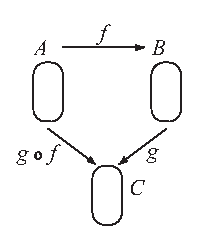
\includegraphics{figps-comparrow.eps}
%\caption{Composition of Functions} \label{fig:functioncomposition2}
\end{center}
\end{figure}

\begin{enumerate}
\item Is it possible to construct an example where  $g \circ f$  is an injection,  $f$  is an injection, but  $g$  is not an injection?  Either construct such an example or explain why it is not possible.

\item Is it possible to construct an example where  $g \circ f$  is an injection,  $g$  is an injection, but  $f$  is not an injection?  Either construct such an example or explain why it is not possible.

\item Is it possible to construct an example where  $g \circ f$  is a surjection,  $f$  is a surjection, but  $g$  is not a surjection?  Either construct such an example or explain why it is not possible.

\item Is it possible to construct an example where  $g \circ f$  is surjection,  $g$  is a surjection, but  $f$  is not a surjection?  Either construct such an example or explain why it is not possible.
\end{enumerate}
%
%\subsection*{Theorems about Composite Functions}\index{composite function!theorems about}
%In the previous two activities, we explored some properties of composite functions related to injections, surjections, and bijections.  The following two theorems contain results that these explorations were intended to illustrate.  Many of the proofs will be included in the exercises.
%
%\begin{theorem} \label{T:compositefunctions}
%Let  $A$, $B$, and  $C$  be nonempty sets and let  $f\x A \to B$ and  $g\x B \to C$.
%
%\begin{enumerate}
%\item If  $f$  and  $g$  are both injections, then  $g \circ f$  is an injection. \label{T:compositefunctions1}
%
%\item If  $f$  and  $g$  are both surjections, then  $g \circ f$  is a surjection. \label{T:compositefunctions2}
%
%\item If  $f$  and  $g$  are both bijections, then  $g \circ f$  is a bijection. \label{T:compositefunctions3}
%\end{enumerate}
%\end{theorem}
%%\hbreak
%%
%The results of Theorem~\ref{T:compositefunctions} are related to the explorations in Activity~\ref{A:compositesofinjections}.  Part~(\ref{T:compositefunctions3}) of Theorem~\ref{T:compositefunctions} is a direct consequence of the first two parts.  We will discuss constructing a proof  of Part~(\ref{T:compositefunctions2}).  Using the forward-backward process, we first look at the conclusion of the conditional statement in Part~(\ref{T:compositefunctions2}).  The goal is to prove that  $g \circ f$  is a surjection.  Since  $g \circ f\x A \to C$, this is equivalent to proving that
%
%\begin{center}
%For all  $c \in C$, there exists an  $a \in A$  such that  
%$( {g \circ f} )( a ) = c$.
%\end{center}
%
%Since this statement in the backward process uses a universal quantifier, we will start by selecting an arbitrary element $c$ in the set $C$.  The goal now is to find an  $a \in A$  such that  $( {g \circ f} )( a ) = c$.
%
%Now we can look at the hypotheses.  In particular, we are assuming that both  $f\x A \to B$  and  $g\x B \to C$  are surjections.  
%
%Since  we have chosen  $c \in C$,  and  $g\x B \to C$  is a surjection, we know that
%
%\begin{center}
%there exists a  $b \in B$  such that  $g( b ) = c$.
%\end{center}
%
%Now, $b \in B$  and   $f\x A \to B$  is a surjection.  Hence
%
%\begin{center}
%there exists an  $a \in A$  such that  $f( a ) = b$.
%\end{center}
%
%If we now compute  $( {g \circ f} )( a )$, we will see that
%\[
%( {g \circ f} )( a ) = g ( f ( a ) ) = g ( b ) = c.
%\]
%We can now write the proof as follows:
%%
%
%\pagebreak
%\noindent
%\textbf{Proof of Theorem~\ref{T:compositefunctions}, Part~(\ref{T:compositefunctions2}).}
%\begin{myproof}
%Let  $A$, $B$, and  $C$  be nonempty sets and assume that  $f\x A \to B$  and  $g\x B \to C$  are both surjections.  We will prove that  $g \circ f\x A \to C$  is a surjection.
%%\vskip10pt
%%\noindent
%
%Let  $c$ be an arbitrary element of  $C$.  We will prove there exists an $a \in A$ such that 
%$( g \circ f ) ( a ) = c$.  Since  $g\x B \to C$  is a surjection, we conclude that
%
%\begin{center}
%there exists a  $b \in B$  such that  $g( b ) = c$.
%\end{center}
%
%\noindent
%Now, $b \in B$  and   $f\x A \to B$  is a surjection.  Hence 
%
%\begin{center}
%there exists an  $a \in A$  such that  $f( a ) = b$.
%\end{center}
%
%\noindent
%We now  see that
%\[
%\begin{aligned}
%  ( {g \circ f} )( a ) &= g( {f( a )} ) \\ 
%                                             &= g( b ) \\ 
%                                             &= c. \\ 
%\end{aligned} 
%\]
%We have now shown that for every  $c \in C$, there exists an  $a \in A$  such that  $( {g \circ f} )( a ) = c$, and this proves that  $g \circ f$  is a surjection.
%\end{myproof}
%\hbreak
%
The results of Theorem~\ref{T:morecompositefunctions} are related to the explorations in Activity~\ref{A:exploringcomposites}.  The proof Theorem~\ref{T:morecompositefunctions} is 
Exercise~(\ref{exer:morecompositefunctions1}).

\begin{theorem} \label{T:morecompositefunctions}
Let  $A$, $B$, and $C$ be nonempty sets and assume that $f\x A \to B$ and  $g\x B \to C$.

\begin{enumerate}
\item If  $g \circ f\x A \to C$  is an injection, then  $f\x A \to B$  is an injection. \label{T:morecompositefunctions1}

\item If  $g \circ f\x A \to C$ is a surjection, then  $g\x B \to C$ is a surjection. \label{T:morecompositefunctions2}
\end{enumerate}
\end{theorem}
\end{activity}
\hbreak










\endinput

\begin{center}
\setlength{\unitlength}{0.5cm}
\begin{picture}(18,14)
\put(2,6.5){\oval(3,11)}
\put(8,6.5){\oval(3,11)}
\put(14,6.5){\oval(3,11)}

\put(2,2){\circle*{.5}}
\put(2,5){\circle*{.5}}
\put(2,8){\circle*{.5}}
\put(2,11){\circle*{.5}}

\put(8,5){\circle*{.5}}
\put(8,8){\circle*{.5}}
\put(8,11){\circle*{.5}}

\put(14,2){\circle*{.5}}
\put(14,5){\circle*{.5}}
\put(14,8){\circle*{.5}}
\put(14,11){\circle*{.5}}

\put(1.1,11){$a$}
\put(1.1,8){$b$}
\put(1.1,5){$c$}
\put(1.1,2){$d$}

\put(8,11.5){$p$}
\put(8,8.5){$q$}
\put(8,5.5){$r$}

\put(14.5,11){$s$}
\put(14.5,8){$t$}
\put(14.5,5){$u$}
\put(14.5,2){$v$}

\put(2,12.5){$A$}
\put(8,12.5){$B$}
\put(14,12.5){$C$}


\put(3,12.8){\vector(1,0){4.7}}
\put(9,12.8){\vector(1,0){4.7}}

\put(5,13.2){$f$}
\put(11,13.2){$g$}

\put(2.5,11){\vector(1,0){5}}
\put(2.5,8){\vector(2,1){5}}
\put(2.5,5){\vector(1,0){5}}
\put(2.5,2.3){\vector(1,1){5.3}}

\put(8.5,10.8){\vector(2,-1){5.2}}
\put(8.5,7.8){\vector(1,-1){5.3}}
\put(8.5,5){\vector(1,0){5}}

\end{picture}
\end{center}

\begin{center}
\setlength{\unitlength}{0.5cm}
\begin{picture}(10,14)
\put(2,6.5){\oval(3,11)}
\put(8,6.5){\oval(3,11)}

\put(2,2){\circle*{.5}}
\put(2,5){\circle*{.5}}
\put(2,8){\circle*{.5}}
\put(2,11){\circle*{.5}}

\put(8,2){\circle*{.5}}
\put(8,5){\circle*{.5}}
\put(8,8){\circle*{.5}}
\put(8,11){\circle*{.5}}

\put(1.1,11){$a$}
\put(1.1,8){$b$}
\put(1.1,5){$c$}
\put(1.1,2){$d$}

\put(8.5,11){$s$}
\put(8.5,8){$t$}
\put(8.5,5){$u$}
\put(8.5,2){$v$}

\put(2,12.5){$A$}
\put(8,12.5){$C$}

\put(3,12.8){\vector(1,0){4.7}}

\put(5,13.2){$g \circ f$}

\put(2.5,11){\vector(2,-1){5}}
\put(2.5,8){\vector(1,0){5}}
\put(2.5,5){\vector(1,0){5}}
\put(2.5,2){\vector(1,0){5}}

\end{picture}
\end{center}

\begin{center}
\setlength{\unitlength}{0.25cm}
\begin{picture}(15,15)
\put(2,10){\oval(2,4)}
\put(10,10){\oval(2,4)}
\put(6,3){\oval(2,4)}

\put(1,12.5){$A$}
\put(9,12.5){$B$}
\put(7.5,3){$C$}


\put(3,13){\vector(1,0){5.5}}
\put(10,7.5){\vector(-4,-3){3.2}}
\put(2,7.5){\vector(4,-3){3.2}}

\put(5.5,13.5){$f$}
\put(8.7,5.5){$g$}
\put(0,5.5){$g \circ f$}


\end{picture}
\end{center}

